\chapter{基于抽象和学习的分布式统计模型检测方法}
\label{ch4}
通过对上一个章节得到的模型进行协同仿真,我们可以得到模型的仿真迹。将仿真迹和需要验证的属性输入到统计模型检测器中,即可以对整个异构系统的行为进行定量的评估分析。但是,由于基于统计模型检测的大型异构系统验证将产生大量的仿真迹,并且每一条迹的产生都十分的耗费时间。因此,使用统计模型检测算法算法对大型异构系统进行验证效率将十分低下。为了解决这一问题,在这一章我们提出了一种基于抽象和学习的分布式统计模型检测方法来提高统计模型检测的效率。本章的第一小节提出了本方法的技术路线及分布式架构设计;第二小节应用分布式架构对一种经典的统计模型检测算法-贝叶斯区间估计算法\cite{zuliani2013bayesian}进行了分布式实现;第三小节首先提出了基于抽象和学习的统计模型检测算法并给出了该算法的分布式实现和优化;最后一个小节给出了基于抽象和学习的分布式统计模型检测算法的算法分析。此外,该算法的效率及准确性对比我们在后面的实验章节给出。
\section{技术路线及分布式架构设计}
在本小节,我们首先给出本方法的技术路线及使用到的分布式架构设计。本方法从在技术上针对两个方面对统计模型检测算法进行改进,并使用了主从式的分布式架构。
\subsection{技术路线}
对统计模型检测算法的效率有直接影响的因素主要有两个:(1)验证过程中产生的仿真迹的数量;(2)产生单条仿真迹需要的时间。在本章,我们针对这两个因素对统计模型检测的效率进行改进。 图\ref{tech-map}是本章的技术路线图,统计模型检测器主要包含三个组件: \emph{仿真器(simulator)、 统计模型检测算法(SMC algorithm)和模型验证器(model checker)}。 \emph{仿真器}产生仿真迹并输入到\emph{模型验证器}之中,\emph{模型验证器}跟根据验证属性来验证该仿真迹是否满足该验证属性,并返回验证结果(返回1表示满足,0表示不满足)。 \emph{统计模型检测算法}收集来自\emph{模型验证器}的验证结果并进行统计分析,最终返回验证结果。为了减少验证过程中产生的仿真迹的数量,我们提出了使用抽象和学习的方法对统计模型检测算法进行改进(AL-SMC),经过多次实验分析,我们发现该方法可以有效减少验证过程中产生的仿真迹。根据论文  \cite{younes2005ymer}, 我们发现统计模型检测算法是可以基于主从架构进行分布式改进的,即可以用多个仿真器产生仿真迹并用一个统计模型检测器进行统计分析,因此,我们可以使用分布式技术来减少产生单条仿真迹需要的时间,并且我们基于分布式技术设计了分布式的贝叶斯区间估计算法。  在本章中,我们结合分布式技术和AL-SMC技术提出了基于抽象和学习的分布式统计模型检测算法(DAL-SMC),该算法同时有效减少了验证过程中产生的仿真迹的数量和产生单条仿真迹需要的时间。
\begin{figure}[htbp]
	{
	\centering	
	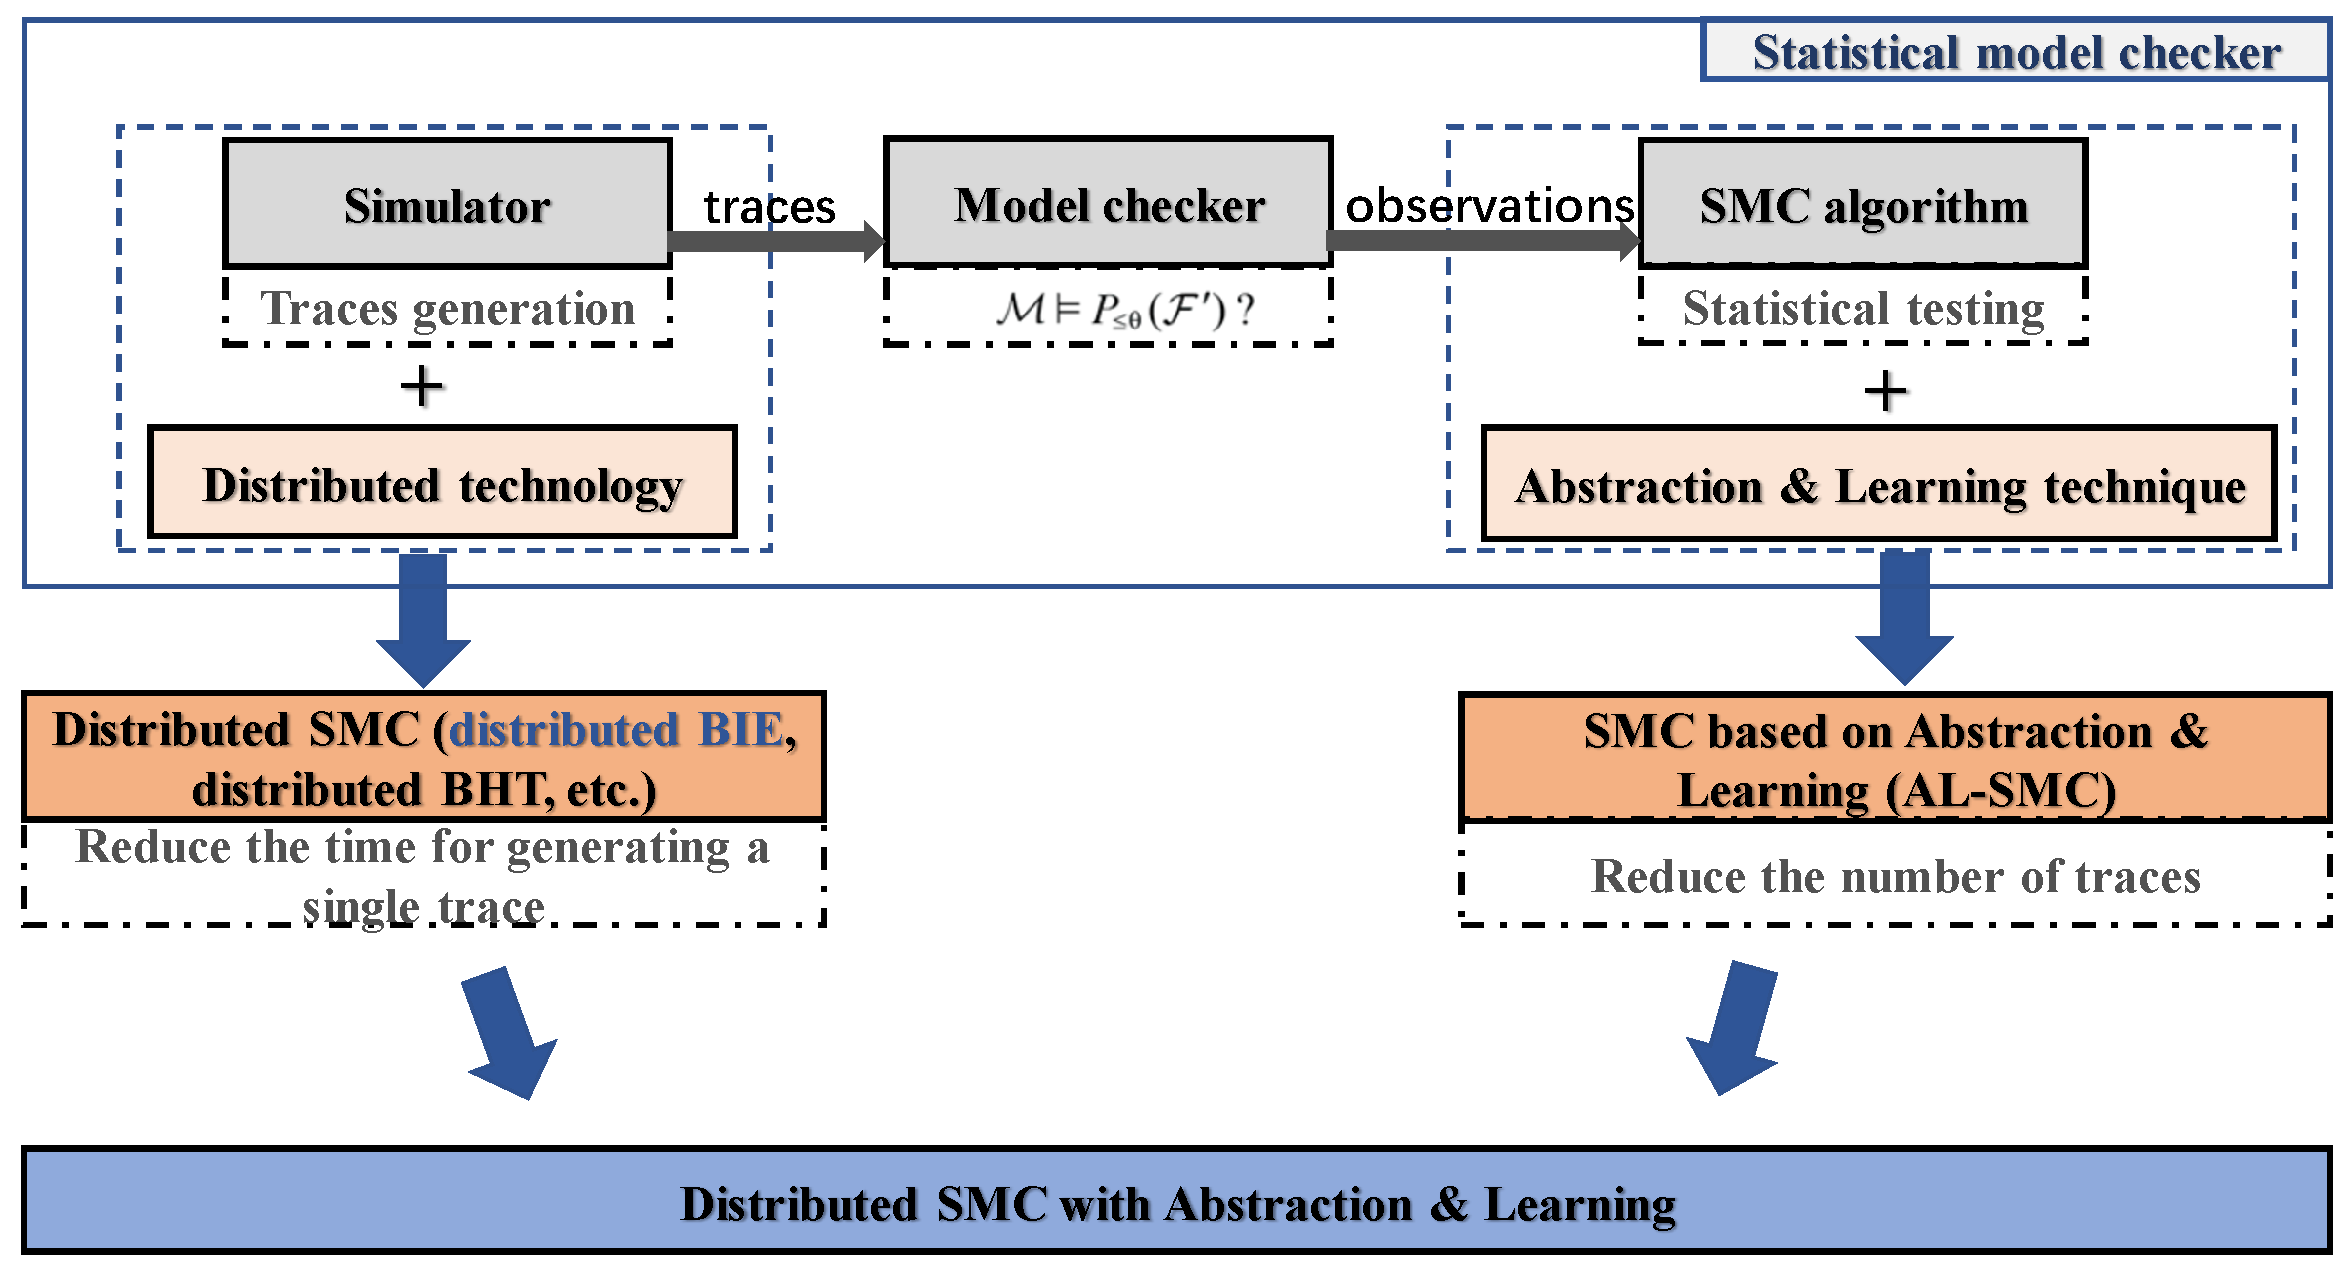
\includegraphics[width=4.0in,height=2.1in]{fig/4/paper-framework.png}
\caption{基于抽象和学习的分布式统计模型检测方法技术路线}\label{tech-map}	
	}	
\end{figure}
\subsection{分布式架构设计}
在本小节,我们给出了统计模型检测算法的分布式架构设计如图\ref{fra}所示:多个从属机器进行模型的仿真并产生仿真迹,然后对该仿真迹进行验证并将验证结果(observation)存储到缓冲器(Buffer)中,主机器从缓冲器中收集验证结果并进行统计分析。在对统计模型检测算法进行分布式改进时,有一个关键点就是要避免引入偏差。为了解决这个问题,我们使用了论文 \cite{Bulychev2012Checking}提出的使用缓冲器和批量处理器来避免偏差的方法。

\begin{figure}[htbp]
\centering{
		\subfigure[分布式架构]{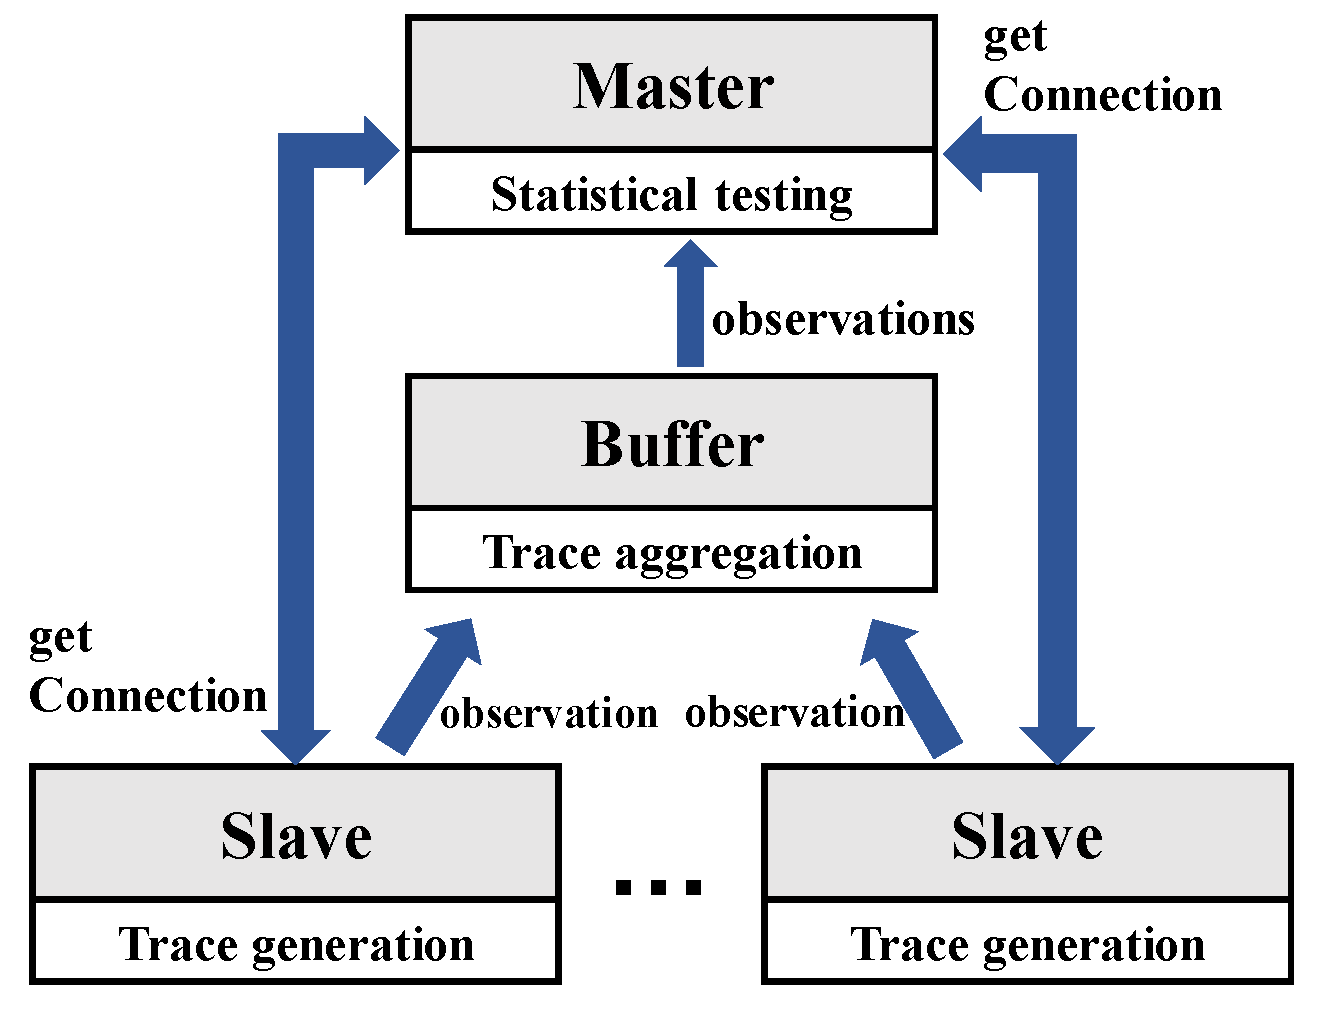
\includegraphics[width=2.5in,height=2.0in]{fig/4/slave-master-ach.png}
			\label{fra}}
		\hfil
		\subfigure[通信协议]{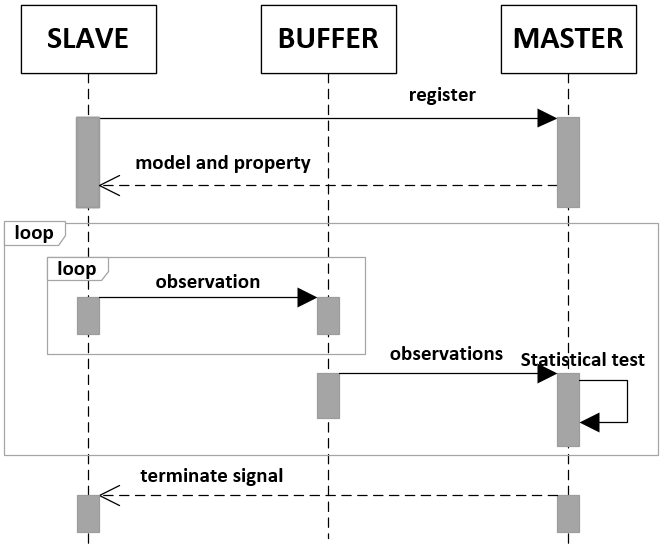
\includegraphics[width=2.5in,height=2.0in]{fig/4/slave-master-seq.png}
			\label{dsmc}}
	\caption{分布式统计模型检测的架构设计}
	\label{fra_dsmc}
	}
\end{figure}
图\ref{dsmc}是分布式统计模型检测的通信协议时序图: (i)多个从属机器跟主机器建立连接,主机器将模型和验证属性发送给从属机器。(ii)从属机器将验证结果发送到缓冲器中,缓冲器中存储的验证结果最终发送到主机器。 (iii)主机器进行统计分析,直到统计分析过程结束,主机器发送终止信号给从属机器,从属机器结束仿真。该分布式统计模型检测算法的框架具有通用性。基于本框架,我们在下个小节设计了分布式的贝叶斯区间估计算法,实际上我们可以将该框架应用到任意一个经典的统计模型检测算法为不只局限于贝叶斯区间估计算法。
\section{分布式的贝叶斯区间估计算法设计}
\subsection{贝叶斯区间估计算法介绍}
\subsection{分布式的贝叶斯区间估计算法}
\section{基于抽象和学习的分布式统计模型检测算法设计}
\subsection{基于抽象和学习的统计模型检测算法}
\subsection{基于抽象和学习的统计模型检测算法的分布式实现}
\subsection{参数优化}
\section{算法分析}
\section{本章小结}
